\documentclass[11pt,a4paper]{article}

\usepackage[utf8]{inputenc}
\usepackage[T1]{fontenc}
\usepackage{lmodern}        % T1 fonts with proper Unicode glyph mapping
\usepackage{cmap}           % embed ToUnicode CMaps -> text is copyable/searchable
\usepackage[margin=2.5cm]{geometry}
\usepackage{graphicx}
\usepackage{float}          % [H] to pin a figure exactly where it is written
\usepackage{booktabs}
\usepackage{longtable}      % tables that break across pages instead of leaving gaps
\usepackage{amsmath}
\usepackage{caption}
\usepackage[hidelinks]{hyperref}
\usepackage[strings]{underscore}
\usepackage{microtype} % tighter justification, fewer over/underfull boxes

% Map font glyphs (incl. ff/fi/fl ligatures) to Unicode so extracted text is correct.
\input{glyphtounicode}
\pdfgentounicode=1

% Let floats fill pages instead of leaving large gaps: allow more of a page to
% be float, tolerate little forced text, and pack figures with surrounding text.
\renewcommand{\topfraction}{0.9}
\renewcommand{\bottomfraction}{0.85}
\renewcommand{\textfraction}{0.07}
\renewcommand{\floatpagefraction}{0.72}
\setcounter{topnumber}{3}
\setcounter{bottomnumber}{2}
\setcounter{totalnumber}{4}

% Discourage orphan/widow lines and page breaks just after a broken word,
% so paragraphs don't strand a single line at the top/bottom of a page.
\clubpenalty=10000
\widowpenalty=10000
\displaywidowpenalty=10000
\brokenpenalty=4000

\title{Remote work, team velocity, and long-term capability\\
       \large An agent-based simulation of a software-development team}
\author{Miłosz Lewandowski\\[4pt]
        \small Source code: \url{https://github.com/milolew/sprint-velocity-simulation}\\[2pt]
        \small Live demo: \href{https://sprint-velocity-simulation-6oaiwsd3eqgf6r3qwfapkz.streamlit.app/}{interactive Streamlit app}}
\date{June 2026}

\begin{document}
\maketitle
% Tighten the gap below the title block without a brittle fixed negative skip.
\vspace{-1.5em plus 0.3em minus 0.3em}

\begin{abstract}
\noindent
This report presents an agent-based model (ABM) of a software-development team built to study how
the share of remote work affects team output and long-term capability. Each developer is an agent
with a per-tick state machine; blockers are resolved either alone or with a colleague's help, and
help between two people in the office is fast and synchronous while any help involving someone at
home is slow and asynchronous. The model is examined at two horizons. Over a \emph{single sprint},
with skill held fixed, velocity falls smoothly with the remote share, and the size of the penalty
depends strongly on how often help is actually needed: $-3.6\%$ for a high-skill team up to
$-13.2\%$ for a team that blocks frequently. Over a \emph{year}, with learning and turnover added,
a co-located team delivers only about $2.5$--$2.8\%$ more cumulative output than a fully remote one,
and, against the naive prior, this penalty is \emph{front-loaded}: it is largest while the team is
junior and shrinks as the team climbs the learning curve. A single-parameter sensitivity analysis
confirms that the average wait for help rises by $59\%$ across the remote range while throughput
falls by only $2.5\%$, and that the most decision-relevant effect of remote work is on the
\emph{spread} of yearly output (roughly tripling), not on its mean. The central conclusion is that
the cost of remote work is not a fixed number but is contingent on the state of the team.
\end{abstract}

\vspace{0.0em}
\begingroup
\setlength{\parskip}{0pt}
\renewcommand{\baselinestretch}{0.80}\selectfont
{\footnotesize\tableofcontents}
\endgroup
\vspace{0.4em}

\section{Introduction}

Whether a software team should work in the office, fully remotely, or somewhere in between is a
recurring management decision, and the evidence behind it is mixed: different studies report
remote work as neutral, mildly harmful, or even helpful for output, and as both good and bad for
retention. A decision-maker therefore needs more than a single average effect; they need to know
\emph{under which conditions} remote work is cheap and under which it is costly.

This report builds an agent-based model to answer that question for one team. The reason for
choosing ABM rather than a regression on aggregate data is that the quantity of interest, team
throughput, emerges from many small, local interactions: an individual developer hits a blocker,
tries to clear it alone, and only then reaches for a colleague, whose availability and location
decide whether the help is fast or slow. These micro-events accumulate into the macroscopic
velocity curve. ABM lets us write down the local rules, which are relatively well understood, and
\emph{observe} the aggregate consequence, which is not. As we will see, the model produces at least
one result that reverses the intuitive prior, which is exactly the kind of non-obvious, emergent
finding that justifies the method.

The single policy variable under study throughout is \texttt{remote\_share}: the probability that
each developer works from home on a given day. Everything else is held at a defensible base case,
and the report asks how output and capability respond as \texttt{remote\_share} is swept from a
fully co-located team ($0$) to a fully remote one ($1$).

The report is organised as follows. Section~\ref{sec:model} describes the model and its per-tick
state machine, and grounds its parameters in the empirical literature. Section~\ref{sec:partA}
measures the direct effect of remote work over a single sprint with skill fixed. Section~\ref{sec:partB}
extends the horizon to a year and adds learning and turnover. Section~\ref{sec:sens} reports a
formal one-parameter sensitivity analysis. Section~\ref{sec:ui} describes the interactive interface,
and Section~\ref{sec:disc} draws the conclusions together.

\section{The model}
\label{sec:model}

\subsection{Overview}

The simulation is built on Mesa~3.x. Time advances in discrete \emph{ticks} of 15 minutes; a working
day is 32 ticks (eight hours) and a sprint of ten working days is 320 ticks. A team of developers
works through a backlog of tasks whose sizes are story points drawn from $\{1,2,3,5\}$, each point
costing four ticks of work by default. Tasks are passive data; the developers are the agents. The
headline experiments use a team of ten developers.

Each morning every developer is independently assigned to the office or to home, with probability
\texttt{remote\_share} of working from home. This single daily coin-flip is the only thing that
\texttt{remote\_share} controls directly; its entire effect on output flows from how that location
choice changes the speed (and, later, the educational value) of help between colleagues.

\subsection{The developer state machine}

The core of the model is a per-tick state machine run by every developer. Its top-level state is one
of \emph{idle}, \emph{working}, \emph{blocked}, or \emph{helping}; while blocked, a secondary stage
(\emph{solo}, \emph{ask\_next\_tick}, \emph{waiting\_for\_help}) tracks how the developer is trying
to get unstuck. Figure~\ref{fig:flow} shows the full cycle.

\begin{figure}[ht]
  \centering
  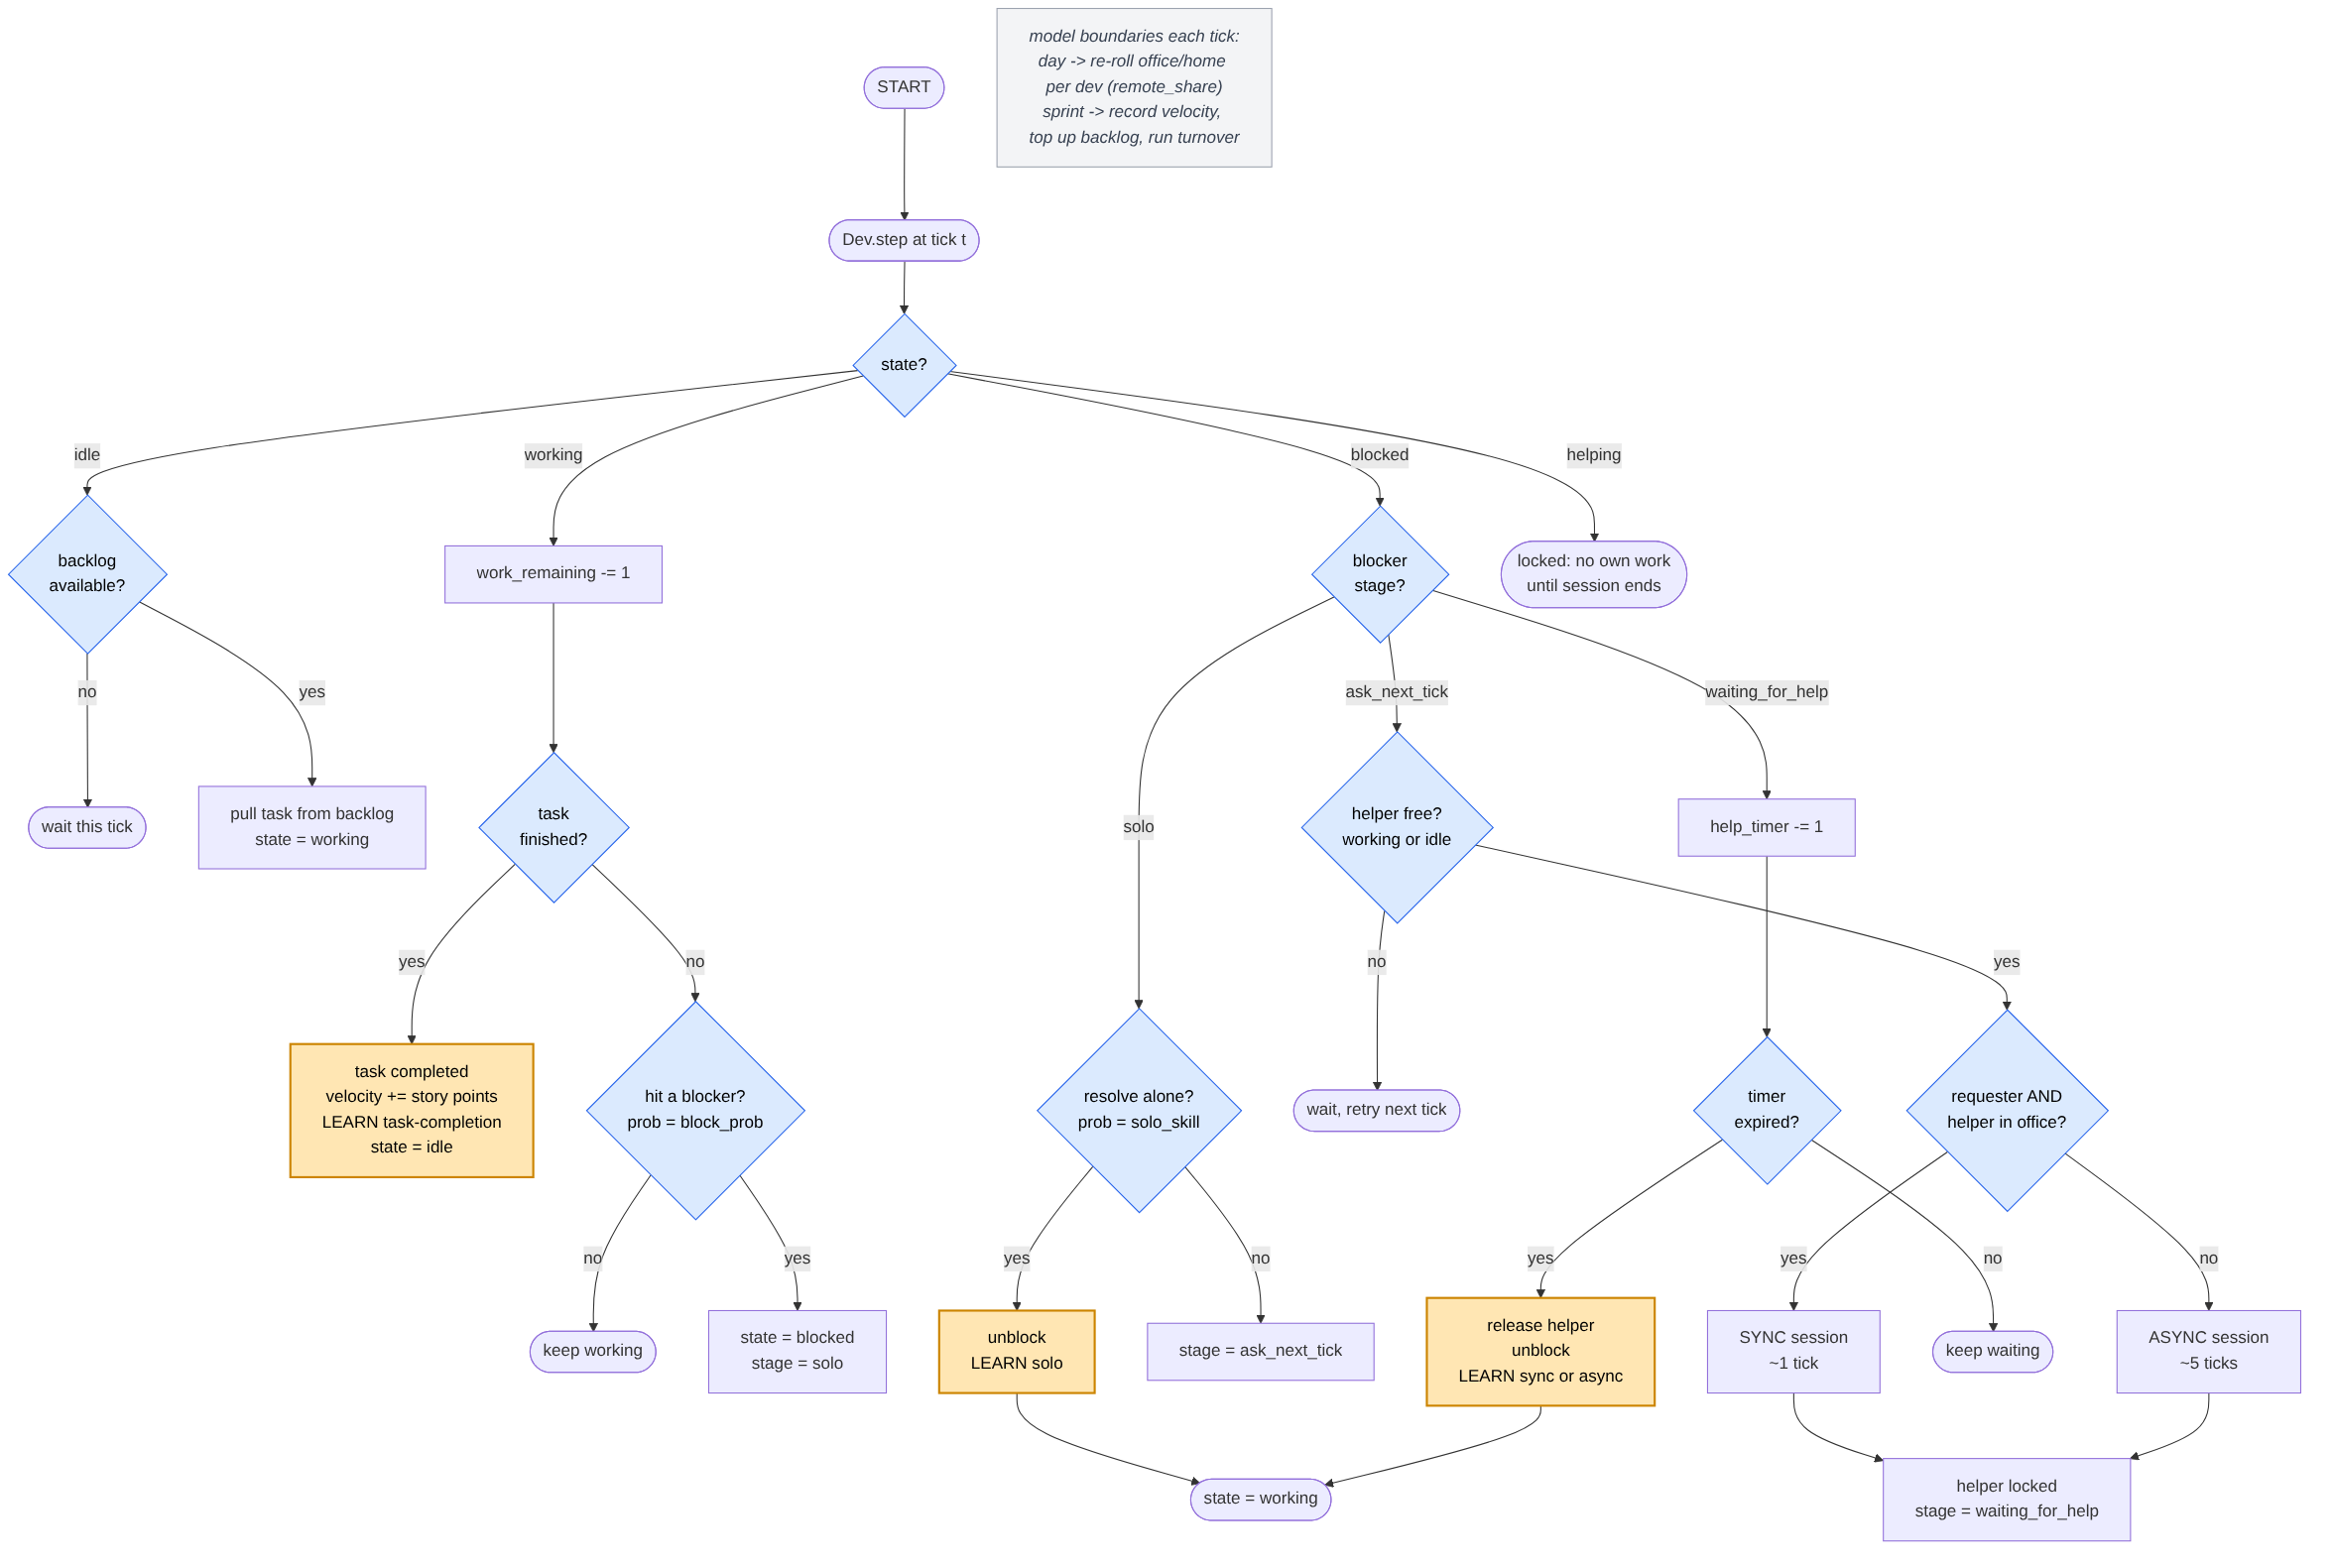
\includegraphics[width=0.93\textwidth]{flowchart_statemachine.png}
  \caption{The per-tick developer state machine. An idle developer pulls work; a working developer
  makes progress and may hit a blocker; a blocked developer first tries to resolve it alone, then
  recruits a helper, opening a fast synchronous session if both are in the office or a slow
  asynchronous one otherwise. Shaded boxes mark \emph{learning events}: the three moments at which a
  developer's skill grows. The note lists the model-level boundaries that wrap the per-agent loop.}
  \label{fig:flow}
\end{figure}

The logic is as follows. An \emph{idle} developer pulls the next task from the backlog and starts
\emph{working}. A \emph{working} developer reduces the task's remaining work by one tick; if the task
is finished it is counted towards velocity and the developer returns to idle, otherwise the developer
may hit a blocker with probability \texttt{block\_prob} on each tick. A \emph{blocked} developer first
attempts a solo resolution, succeeding with probability equal to their individual \emph{solo skill}.
On failure they look, on the next tick, for an available colleague (one who is working or idle).
If a developer in the office finds an office colleague the help is \emph{synchronous} and short
($1\pm1$ ticks); if either party is at home it is \emph{asynchronous} and long ($5\pm2$ ticks). The
helper is locked for the duration of the session and cannot do their own work, which is the channel
through which one person's blocker reduces the whole team's throughput. When no helper is free the
developer simply waits and retries; this is a deliberate throughput limit, not a modelling oversight.

This single distinction, that synchronous, co-located help is roughly five times faster than
asynchronous, remote help, is the entire mechanism by which remote work affects a sprint's output.
Everything in Part~A follows from it.

\subsection{Learning}

Over a single sprint it is reasonable to treat each developer's solo skill as fixed, but over a year
it is not, because people get better at their work. In the extended model, solo skill is the
probability of clearing a blocker alone, and it grows with experience. Every time a developer
completes a task or resolves a blocker, their skill takes a small, deterministic step towards a
ceiling \texttt{skill\_cap}, and the steps shrink as the ceiling approaches:
\[
\text{skill} \;\leftarrow\; \text{skill} \;+\; \texttt{learning\_rate}\cdot w \cdot
(\texttt{skill\_cap} - \text{skill}),
\]
where $w$ is a weight that depends on \emph{how} the experience was gained. This diminishing-returns
form produces fast early progress and then a plateau, matching the empirical onboarding pattern in
which a new hire reaches most of their productivity within roughly six months.

The weight $w$ is where remote work re-enters. Resolving a blocker through co-located help teaches
more than resolving the same blocker asynchronously ($\texttt{sync\_help\_weight}=1.5$ versus
$\texttt{async\_help\_weight}=1.0$). This is the only route by which remote work slows learning, so
the model needs no separate ``remote learning'' switch. Crucially, most learning weight comes from
ordinary task completion, which is location-independent; the location-dependent mentoring bonus
applies only to the rarer blocker-resolution events.

\subsection{Turnover}

At the end of each sprint every developer may leave, with a per-sprint hazard derived from an annual
attrition rate (about $12\%$ per year in the base case). Anyone who leaves is replaced immediately by
a junior who starts at low skill and must learn from scratch; any partly finished task they held
returns to the backlog with its progress lost. Each departure therefore pulls the team's mean skill
down and resets part of the learning curve.

Remote work can raise or lower the chance of leaving through a single coefficient,
\texttt{remote\_attrition\_coef}. Because the empirical sign is genuinely contested (one large
randomized trial finds remote work \emph{improves} retention, while a natural experiment finds lost
in-person mentorship \emph{raises} junior quitting), the coefficient defaults to zero and results are
reported under both readings. This contested knob is the headline decision-support lever of the model.

\subsection{Parameters and their empirical grounding}

The model's parameters are not guessed; each is a defensible synthesis of published evidence,
intended as a sensitivity-analysis base case rather than a precise constant. Table~\ref{tab:params}
lists the load-bearing ones with their values, ranges, and the strength of the evidence behind them.
No source measures the model's exact constructs (population-level voluntary developer turnover, or
the probability of resolving a blocker solo as a function of tenure), so every value is a
reconstruction from adjacent measures, and the report relies on sweeps rather than on any single
point estimate.

\begin{table}[H]
\centering
\caption{The load-bearing parameters, their base-case values, and their empirical grounding.}
\label{tab:params}
\small
\setlength{\tabcolsep}{4pt}
\begin{tabular}{lllp{5.6cm}}
\toprule
Parameter & Base case & Sweep / range & Grounding (evidence strength) \\
\midrule
\texttt{remote\_share}          & 0.5         & 0--1            & Policy variable under study. \\
\texttt{block\_prob}            & 0.02 / tick & 0.01--0.05      & Process rate; swept as a moderator. \\
\texttt{mean\_solo\_skill}      & 0.5         & 0.3--0.7        & Team-mean blocker self-resolution. \\
\texttt{sync\_help\_mean}       & 1 tick      & fixed           & Co-located help is fast. \\
\texttt{async\_help\_mean}      & 5 ticks     & fixed           & Remote help $\sim 5\times$ slower (async). \\
\texttt{annual\_attrition}      & 0.12        & 0.08--0.20      & Med: $\sim$10--15\%/yr developer voluntary turnover; no clean source. \\
\texttt{skill\_cap}             & 0.90        & 0.85--0.95      & High: early hard plateau (3 independent sources). \\
\texttt{junior\_mean\_skill}    & 0.40$\times$cap & 0.35--0.50  & Med: reconstructed from expert/novice $\sim$2:1. \\
\texttt{learning\_rate}         & 0.0123      & calibrated      & Med: fitted so a junior closes $\sim$90\% of the gap in $\sim$6 months. \\
\texttt{sync\,:\,async\_weight} & 1.5 : 1.0   & 1.2$\times$--2$\times$ & High (general), Low (junior multiplier): co-located mentoring premium. \\
\texttt{remote\_attrition\_coef}& 0.0         & $-1$ \ldots $+1$ & High both arms, sign contested (retention vs.\ isolation). \\
\bottomrule
\end{tabular}
\end{table}

The learning rate deserves a note because it is the one parameter fitted by the model itself rather
than read off the literature. It was calibrated by simulation so that a junior closes about $90\%$ of
the gap to the skill ceiling in roughly twelve sprints ($\sim$6 months), the modal ramp-up time in
onboarding studies; the bisection result $\texttt{learning\_rate}=0.0123$ agrees with an independent
analytic cross-check. The fitted rate reproduces the documented ramp: $68\%$ of the gap closed by
three months, $90\%$ by six, $99\%$ by twelve.

\section{Part A: a single sprint}
\label{sec:partA}

Part~A holds each developer's skill fixed and measures the direct effect of remote work on one
sprint's velocity. Three experiment series were run, each with 20 replications (different random
seeds) per cell, for 940 simulations in total. The remaining parameters keep their defaults: office
help takes $1\pm1$ ticks, remote help $5\pm2$ ticks, and individual solo skill is spread by $\pm0.2$
around its mean.

\begin{center}
\setlength{\tabcolsep}{4pt}
\begin{tabular}{clccc}
\toprule
\# & Factor(s) & Levels & Replications & Total runs \\
\midrule
1 & \texttt{remote\_share} (baseline)            & 11 (0.0--1.0, step 0.1)        & 20 & 220 \\
2 & \texttt{remote\_share} $\times$ \texttt{mean\_solo\_skill} & $6\times3$ (skill $0.3,0.5,0.7$) & 20 & 360 \\
3 & \texttt{remote\_share} $\times$ \texttt{block\_prob}      & $6\times3$ (bp $0.01,0.02,0.05$)  & 20 & 360 \\
\bottomrule
\end{tabular}
\end{center}

\subsection{Experiment 1: baseline sweep}

As the share of remote work rises from none to everyone, velocity falls steadily and the average
wait for help grows, because more of the help that does happen is the slower, asynchronous kind
(Figure~\ref{fig:exp1}). The fall is smooth: there is no threshold or sudden collapse.

\begin{figure}[ht]
  \centering
  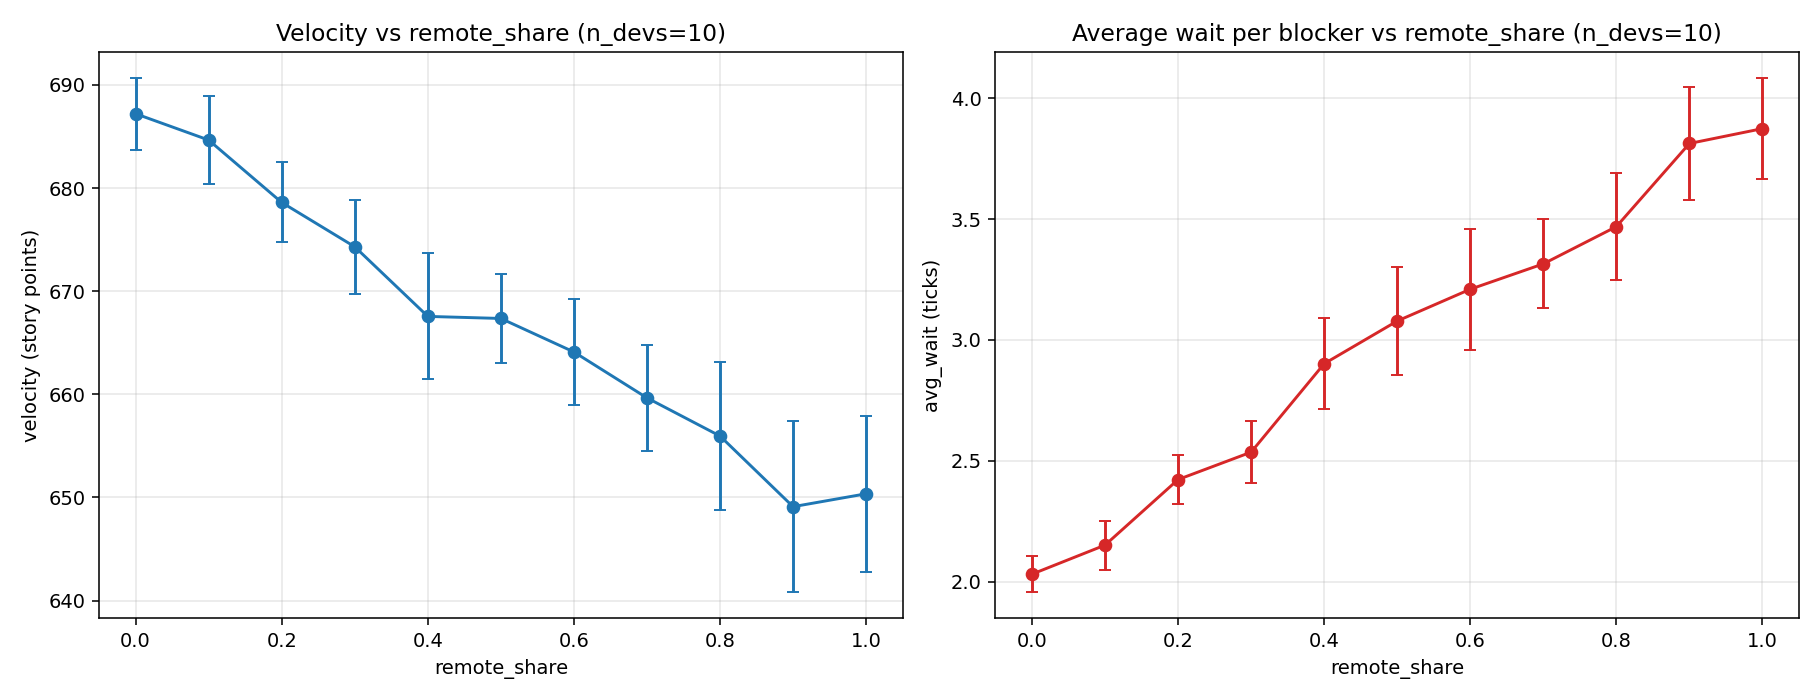
\includegraphics[width=0.80\textwidth]{exp1_baseline.png}
  \caption{Velocity and average wait per blocker against the share of remote work, baseline sweep
  (10 developers, 20 replications per level, 95\% confidence intervals).}
  \label{fig:exp1}
\end{figure}

\begin{center}
\begin{tabular}{cccc}
\toprule
\texttt{remote\_share} & velocity (mean $\pm$ CI95) & avg.\ wait & blockers resolved \\
\midrule
0.0 & $687.2 \pm 3.5$ & 2.0 & 52.0 \\
0.3 & $674.3 \pm 4.6$ & 2.5 & 52.3 \\
0.5 & $667.4 \pm 4.3$ & 3.1 & 49.2 \\
0.7 & $659.6 \pm 5.2$ & 3.3 & 50.6 \\
1.0 & $650.4 \pm 7.6$ & 3.9 & 47.5 \\
\bottomrule
\end{tabular}
\end{center}

\subsection{Experiment 2: remote share and individual skill}

The size of the remote penalty depends on how often people actually need help. A more skilled team
clears most blockers alone and barely notices slower remote help; a less skilled team leans on the
help channel and suffers far more. The velocity lost when moving from a fully office to a fully
remote team ranges from $9.0\%$ for a low-skill team down to $3.6\%$ for a high-skill one
(Figure~\ref{fig:exp2}).

\begin{figure}[ht]
  \centering
  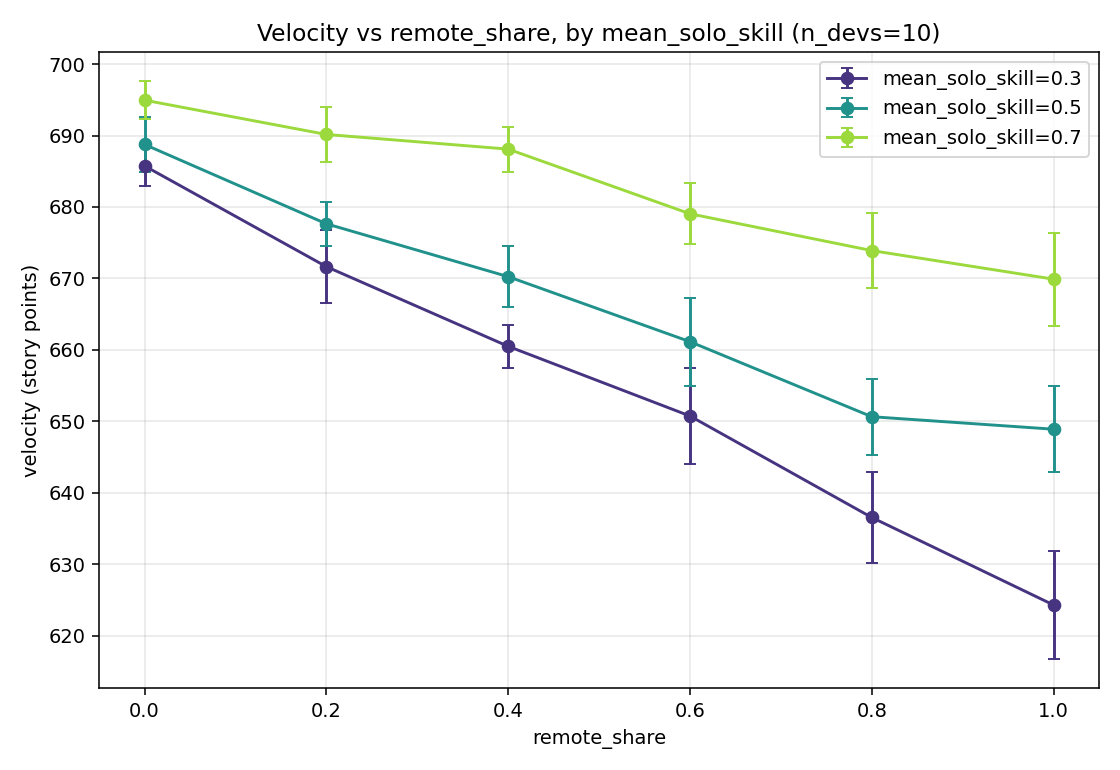
\includegraphics[width=0.58\textwidth]{exp2_skill_interaction.png}
  \caption{Velocity against remote share, grouped by mean solo skill.}
  \label{fig:exp2}
\end{figure}

\begin{center}
\begin{tabular}{ccccc}
\toprule
\texttt{mean\_solo\_skill} & velocity @ 0\,\% & velocity @ 100\,\% & absolute loss & relative loss \\
\midrule
0.30 & 685.8 & 624.3 & $-61.5$ SP & $-9.0\%$ \\
0.50 & 688.8 & 648.9 & $-39.9$ SP & $-5.8\%$ \\
0.70 & 695.0 & 669.9 & $-25.1$ SP & $-3.6\%$ \\
\bottomrule
\end{tabular}
\end{center}

\subsection{Experiment 3: remote share and blocker frequency}

For the same reason, the penalty grows sharply with how often blockers occur. When blockers are rare
the help channel is used little and remote work costs about $3\%$; when they are frequent the team is
constantly waiting for help and the cost rises to roughly $13\%$ (Figure~\ref{fig:exp3}). Experiments
2 and 3 tell one story from two directions: the remote penalty is a tax on the help channel, so it
scales with how heavily that channel is used.

\begin{figure}[ht]
  \centering
  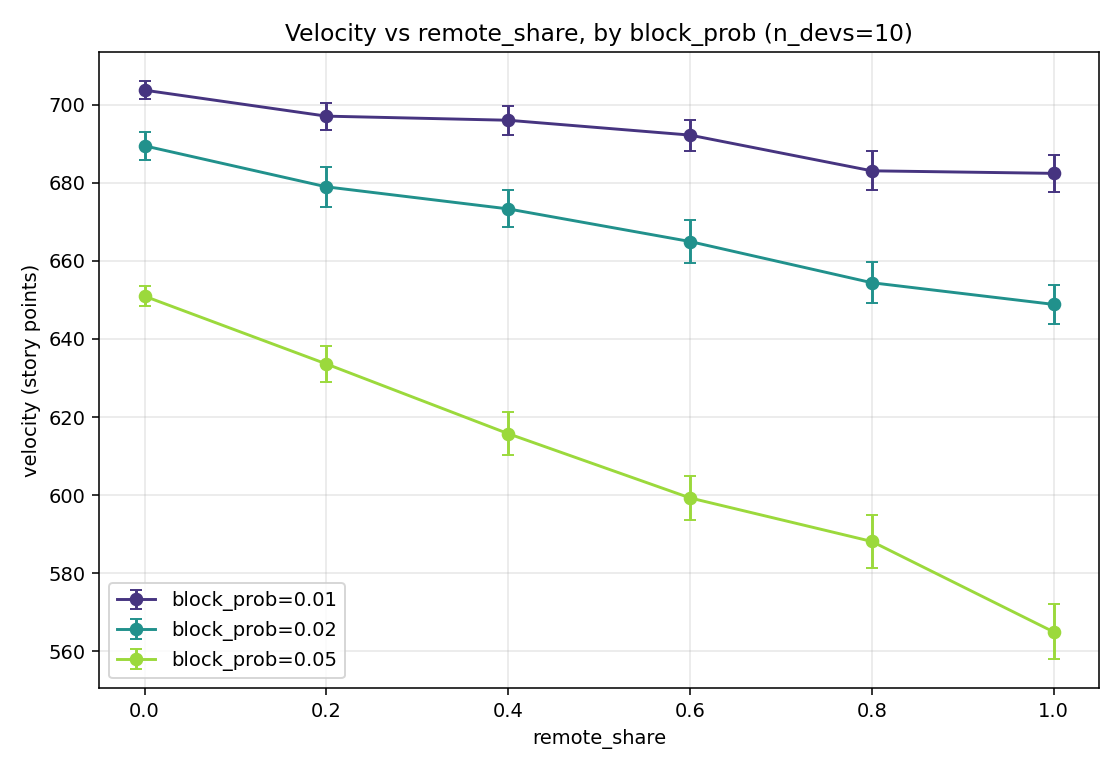
\includegraphics[width=0.58\textwidth]{exp3_blockprob_interaction.png}
  \caption{Velocity against remote share, grouped by blocker probability.}
  \label{fig:exp3}
\end{figure}

\begin{center}
\begin{tabular}{ccccc}
\toprule
\texttt{block\_prob} & velocity @ 0\,\% & velocity @ 100\,\% & absolute loss & relative loss \\
\midrule
0.01 & 703.7 & 682.4 & $-21.3$ SP & $-3.0\%$ \\
0.02 & 689.5 & 648.9 & $-40.6$ SP & $-5.9\%$ \\
0.05 & 651.0 & 565.0 & $-86.0$ SP & $-13.2\%$ \\
\bottomrule
\end{tabular}
\end{center}

\section{Part B: a year, with learning and turnover}
\label{sec:partB}

Part~A treats skill as fixed, which is fine for one sprint but not for a year, over which people get
better and teams lose and gain members. Part~B turns on learning and turnover and runs the model over
24 two-week sprints ($\sim$1 year). The measure that matters here is \emph{cumulative velocity}: the
total story points delivered over the whole year, not in any single sprint. Four sweeps of the remote
share were run, again with 20 replications per cell.

\subsection{The remote penalty is front-loaded, not compounding}

Across the year a fully co-located team delivers roughly $2.5$--$2.8\%$ more than a fully remote one.
The gap grows monotonically with the remote share, but its most telling feature is \emph{when} it
occurs: it is largest early in the year and shrinks as the team matures.

\begin{center}
\begin{tabular}{lc}
\toprule
Horizon & Advantage of the office team \\
\midrule
6 sprints (about 3 months)  & $+4.7\%$ \\
12 sprints (about 6 months) & $+3.3\%$ \\
24 sprints (about 1 year)   & $+2.6\%$ \\
\bottomrule
\end{tabular}
\end{center}

It was natural to expect the opposite: that a small per-sprint penalty would \emph{compound} as the
two teams' skills diverged over the year. The model shows the reverse, and the reason is instructive.
The remote penalty is at heart a penalty on the help channel: remote developers wait longer for
asynchronous help. Learning works \emph{against} this penalty rather than with it. As both teams grow
more skilled they need help less often, so the channel where remote work loses ground matters less
and less. With learning switched off, the office team's advantage over a year is $6.2\%$; with
learning on it falls to $2.5\%$ (Figure~\ref{fig:penalty}). The cost of remote work is concentrated
in the early, junior, frequently-blocked phase and fades once the team is experienced.

\begin{figure}[ht]
  \centering
  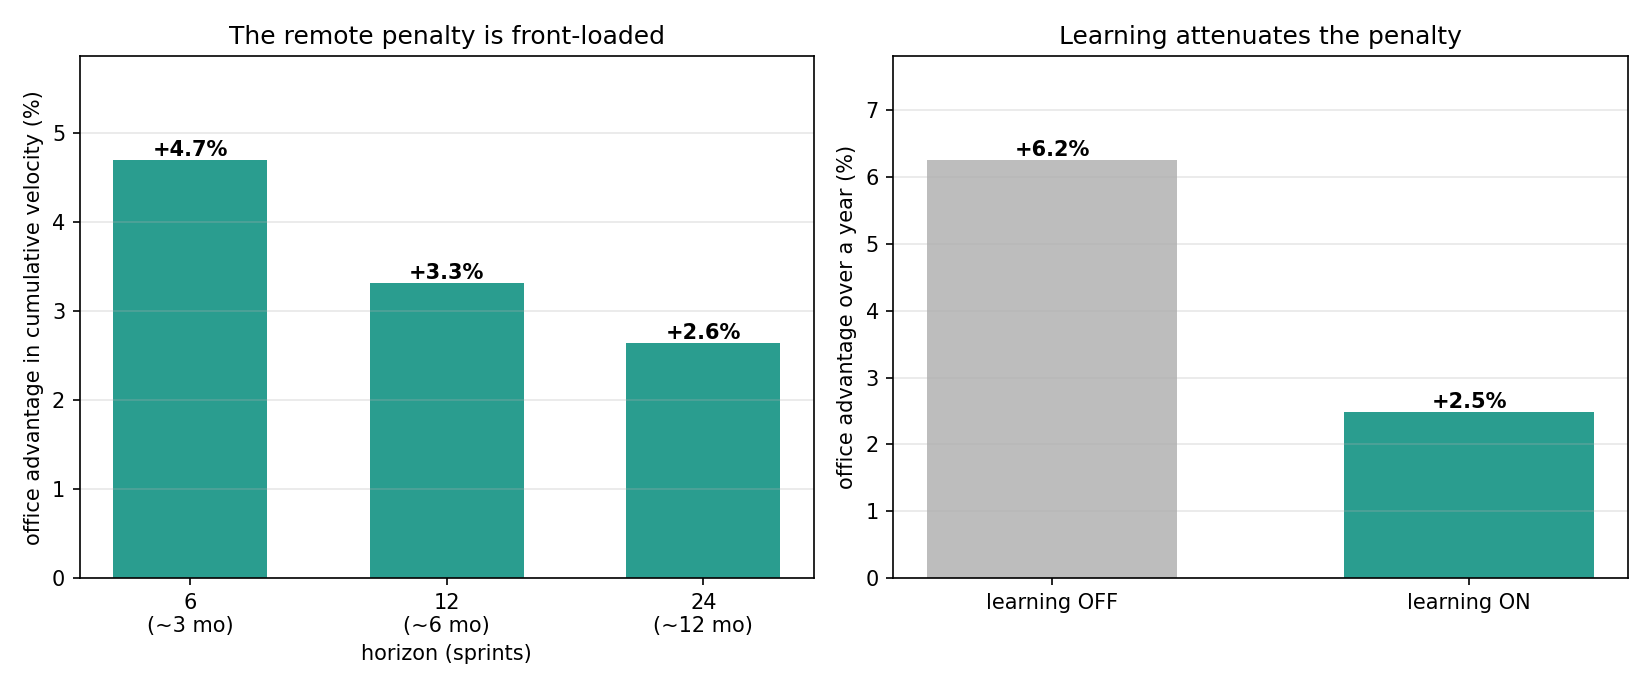
\includegraphics[width=0.88\textwidth]{partb_penalty.png}
  \caption{The office advantage in cumulative velocity is largest early and shrinks over the year
  (left); switching learning on more than halves it (right).}
  \label{fig:penalty}
\end{figure}

The skill ramp makes the mechanism visible (Figure~\ref{fig:ramp}). For a team that starts as
juniors, the office team ramps a little faster, but both reach the same ceiling, so the office/remote
skill gap is widest mid-ramp and closes by year end. This is why the penalty shows up in ramp speed
and cumulative output, not in the end-of-year skill level.

\begin{figure}[ht]
  \centering
  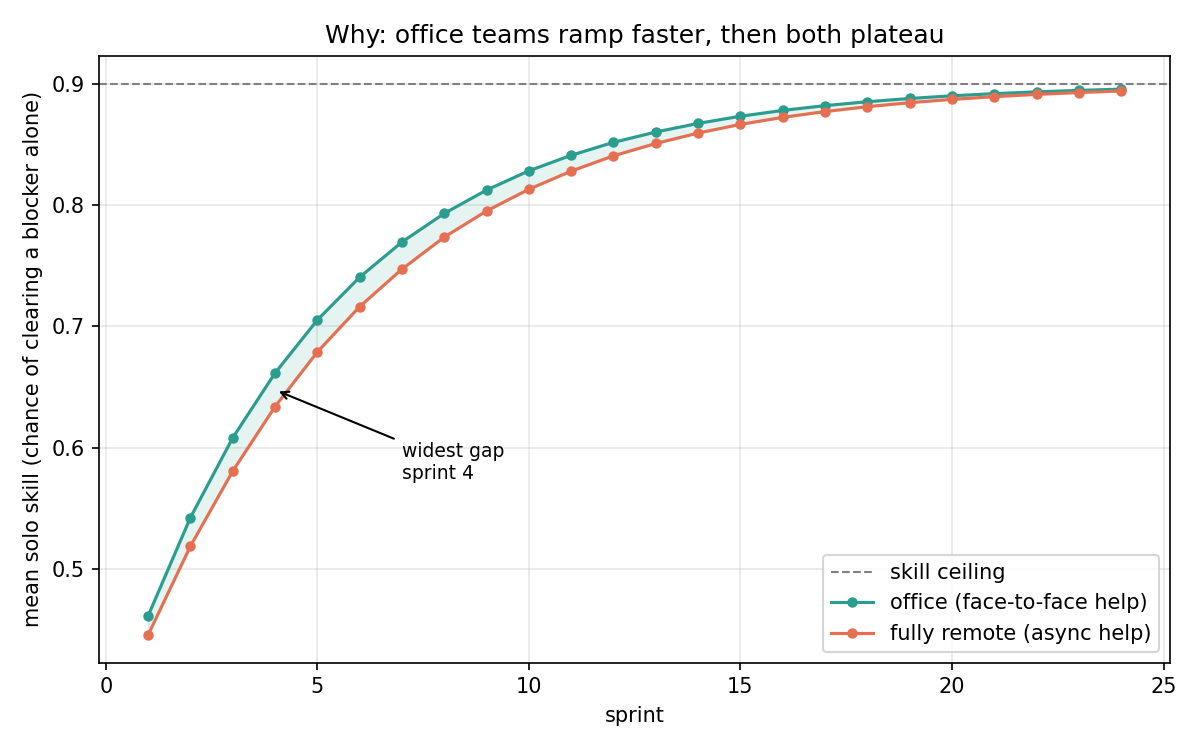
\includegraphics[width=0.55\textwidth]{partb_skillramp.png}
  \caption{Mean solo skill over the year for a team of juniors. The office team ramps slightly
  faster, but both converge to the same plateau.}
  \label{fig:ramp}
\end{figure}

\subsection{Turnover reproduces both literature scenarios}

The turnover coefficient behaves as designed. Under the \emph{retention} reading, where remote work
helps keep people, a fully remote team loses fewer members over the year than an office team; under
the \emph{isolation} reading, where remote work pushes juniors out, it loses more
(Figure~\ref{fig:turnover}). Reporting both arms, rather than picking one, is the core
decision-support output of the model, because the empirical sign is genuinely unresolved.

\begin{center}
\begin{tabular}{ll}
\toprule
Scenario & departures: office $\to$ fully remote \\
\midrule
retention (remote keeps people)   & $1.9 \to 0.7$ \\
isolation (remote pushes them out) & $0.6 \to 2.0$ \\
\bottomrule
\end{tabular}
\end{center}

\begin{figure}[ht]
  \centering
  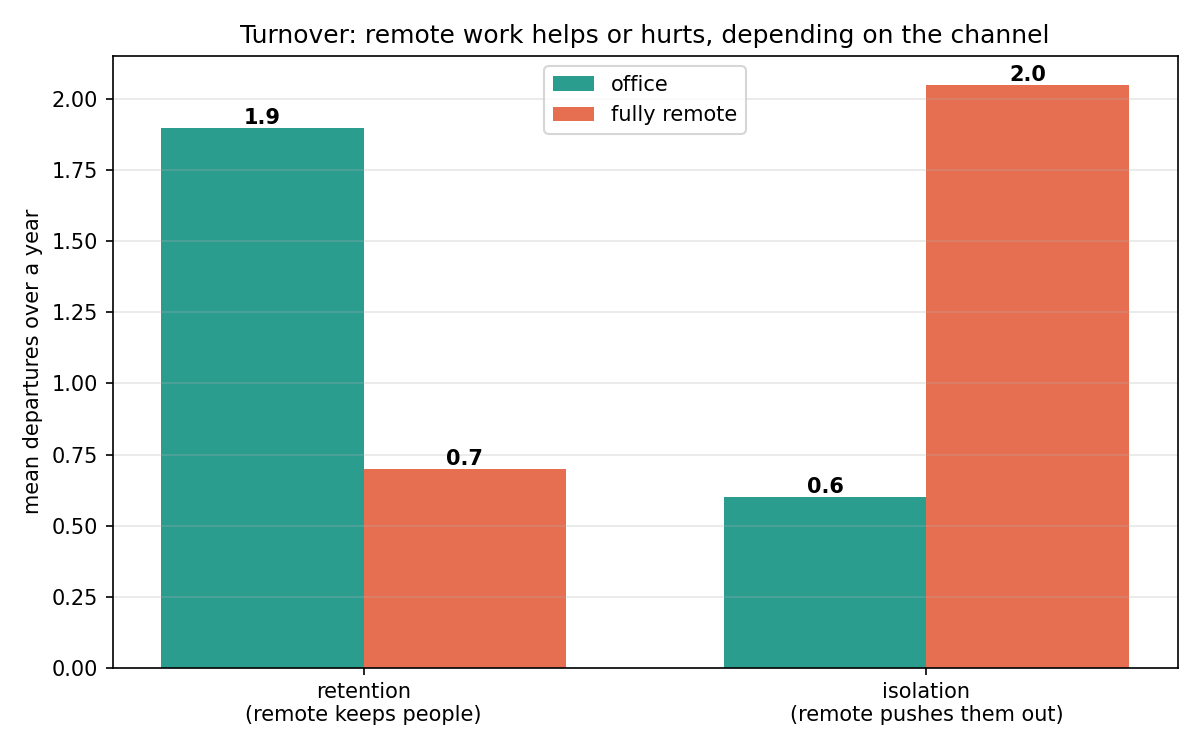
\includegraphics[width=0.55\textwidth]{partb_turnover.png}
  \caption{Departures over a year, office versus fully remote, under the two readings of how remote
  work affects retention.}
  \label{fig:turnover}
\end{figure}

Under immediate junior replacement, turnover is nearly velocity-neutral within a single year, so its
signal lives in the departure count rather than in throughput. Over multiple years, however, a
departure that swaps a senior for a junior would feed back into the skill channel, so even a moderate
effect through \texttt{remote\_attrition\_coef} would plausibly outweigh the $2.5\%$ throughput effect
studied here.

\section{Sensitivity analysis of \texttt{remote\_share}}
\label{sec:sens}

To put the headline parameter on a firmer footing, a formal one-parameter sensitivity study was run
in the year-long regime (24 sprints, learning and turnover on, all other parameters at their
defaults). \texttt{remote\_share} was swept across its full range $[0,1]$ in steps of $0.05$, with
80 repetitions per level; a separate sub-study with 400 repetitions at three levels was used to check
how many repetitions are needed.

\subsection{How many repetitions are enough}

The number of repetitions needed is not the same for every quantity (Figure~\ref{fig:conv}). A full
year averages over many thousands of small events, so the mean of yearly throughput settles quickly:
about 40 repetitions give it to within $\pm0.1\%$, and 80 give $\pm0.08\%$ even at the noisiest end of
the range. A count of rare events behaves very differently. The attrition count has a mean near $1.1$
and a standard deviation near $1.0$, so its relative error is still about $\pm20\%$ at 80 repetitions.
Eighty repetitions are therefore ample for the throughput results, but a rare-event count would need
several hundred.

\begin{figure}[ht]
\centering
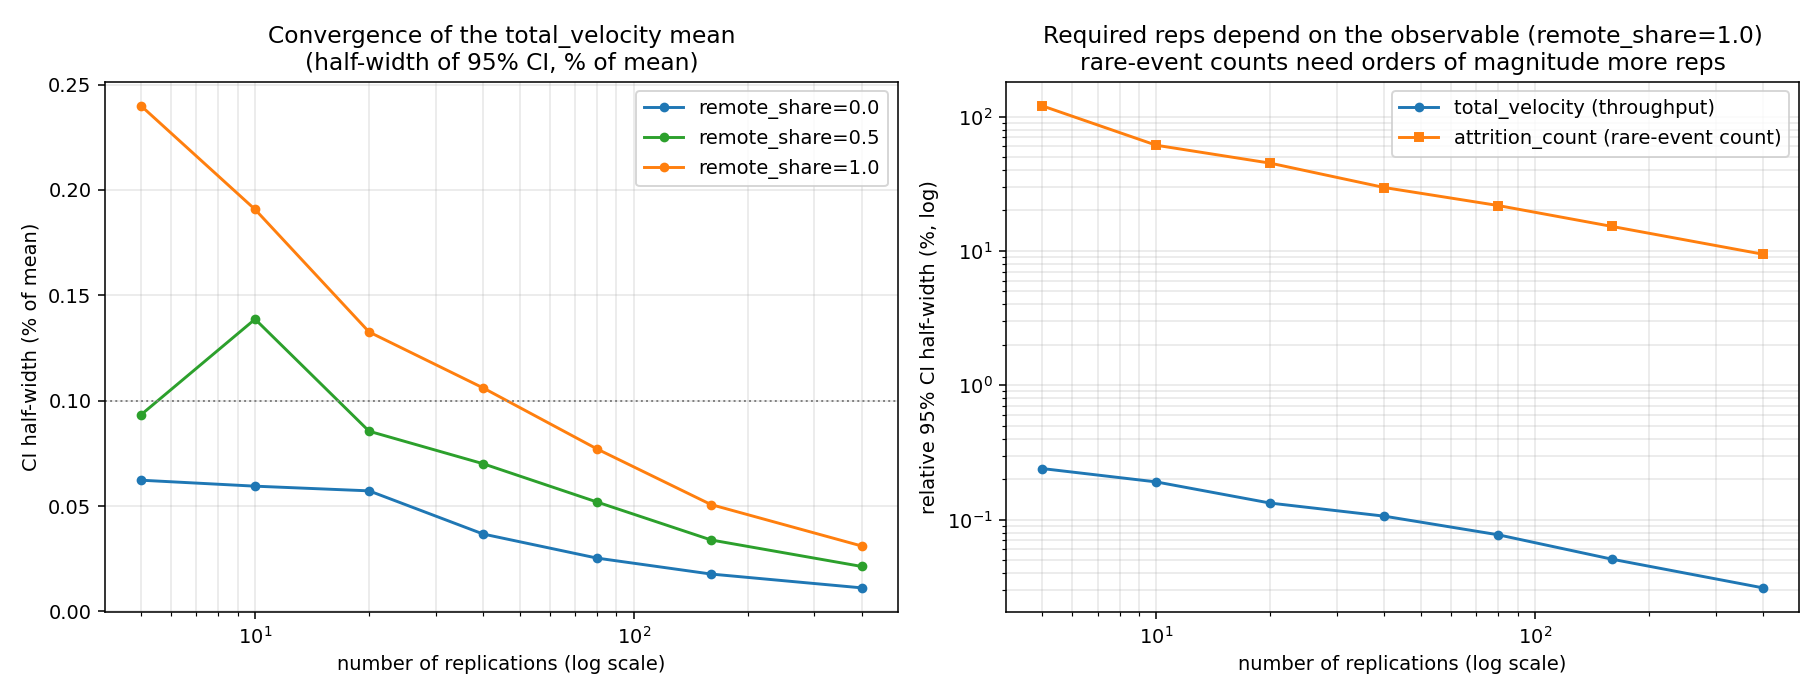
\includegraphics[width=0.62\textwidth]{sens_fig4_convergence.png}
\caption{Width of the 95\% confidence interval against the number of repetitions. Throughput (left)
settles quickly; the attrition count (right) needs far more runs for the same relative precision.}
\label{fig:conv}
\end{figure}

\subsection{The mean moves little; the spread moves a lot}

Throughput goes down as remote work increases, but only by about $2.5\%$ across the full range, with
no sudden jump. The mechanism behind it changes much more: the average wait per blocker rises by
$59\%$ (Figure~\ref{fig:rel}), because help involving someone at home is asynchronous and roughly
five times slower. The two are loosely linked because blockers are rare next to ordinary work: the
extra waiting amounts to about a thousand idle ticks against roughly $77{,}000$ working ticks in the
year, close to $1.3\%$, the same order of magnitude as the throughput drop. The parameter that looks
most important in the mechanism is therefore not the one that controls the final result.

\begin{figure}[ht]
\centering
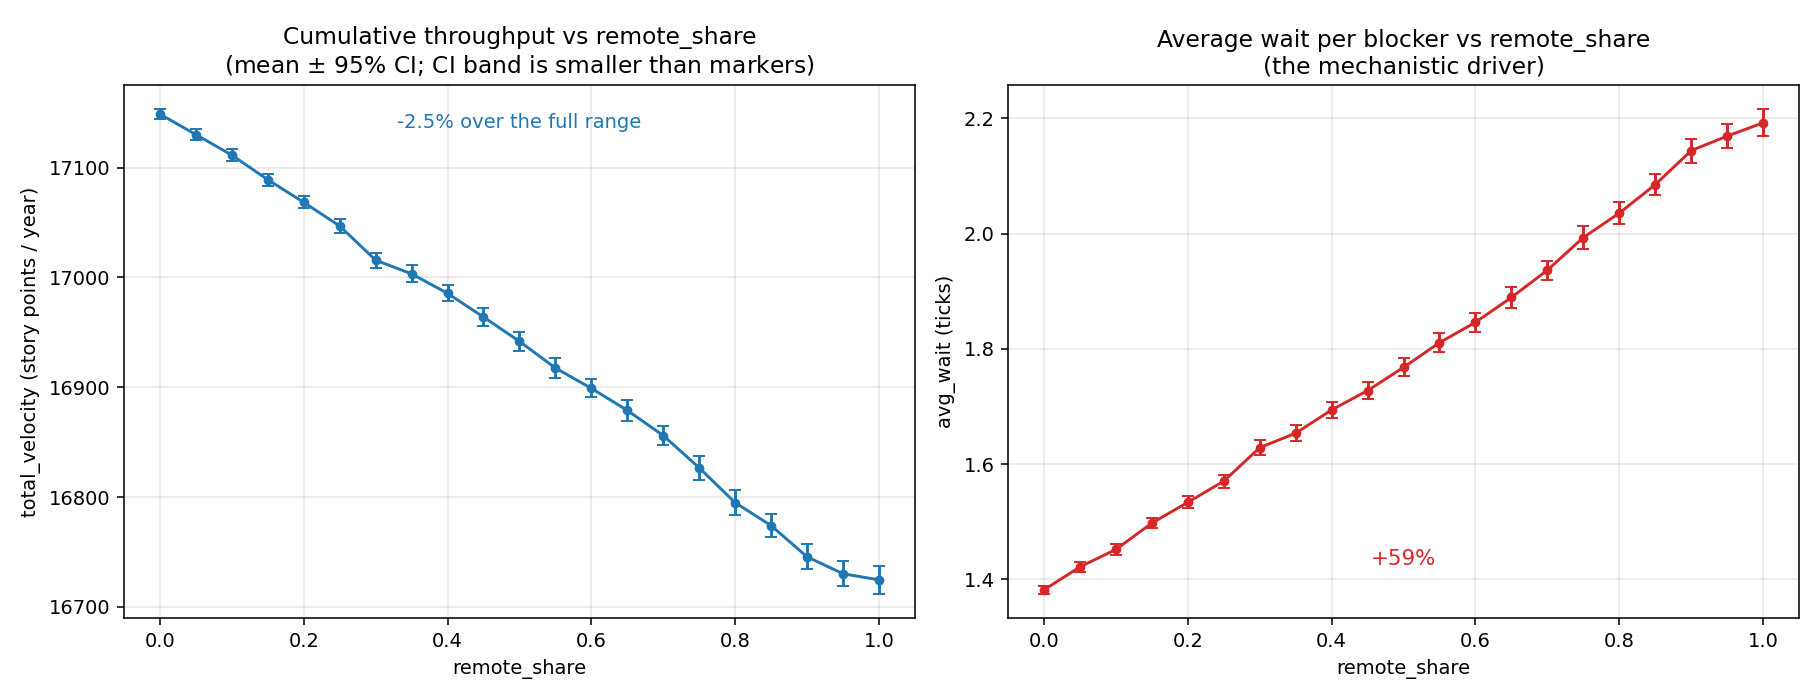
\includegraphics[width=0.62\textwidth]{sens_fig1_relationship.png}
\caption{Yearly throughput falls by $2.5\%$ across the full range (left), while the average wait per
blocker rises by $59\%$ (right). Means with 95\% confidence intervals, 80 repetitions per point.}
\label{fig:rel}
\end{figure}

The mean alone, however, hides the most decision-relevant effect. Keeping the full set of run results
rather than reducing each level to an average (Figure~\ref{fig:disp}) shows that the spread of yearly
throughput grows about threefold as remote work increases (the run-to-run standard deviation rises
from about 20 to 59 story points), while the mean moves by only $2.5\%$. In other words, how
\emph{predictable} the output is depends on remote work far more strongly than the average output
does. An analysis that looked only at the mean would miss this entirely.

Two further results are worth stating. First, remote work does not reduce end-of-year skill, which
stays flat near $0.88$ across the whole range, because most learning comes from finishing tasks
(location-independent) and the in-office mentoring bonus applies only to the rarer blocker-resolution
events. Second, the attrition count shows no trend with \texttt{remote\_share}, but only because the
default \texttt{remote\_attrition\_coef}$=0$ severs the link by construction. That flat result is an
honest caveat, not a finding, and sweeping the coefficient over $[-1,1]$ is the natural next step.

\begin{figure}[ht]
\centering
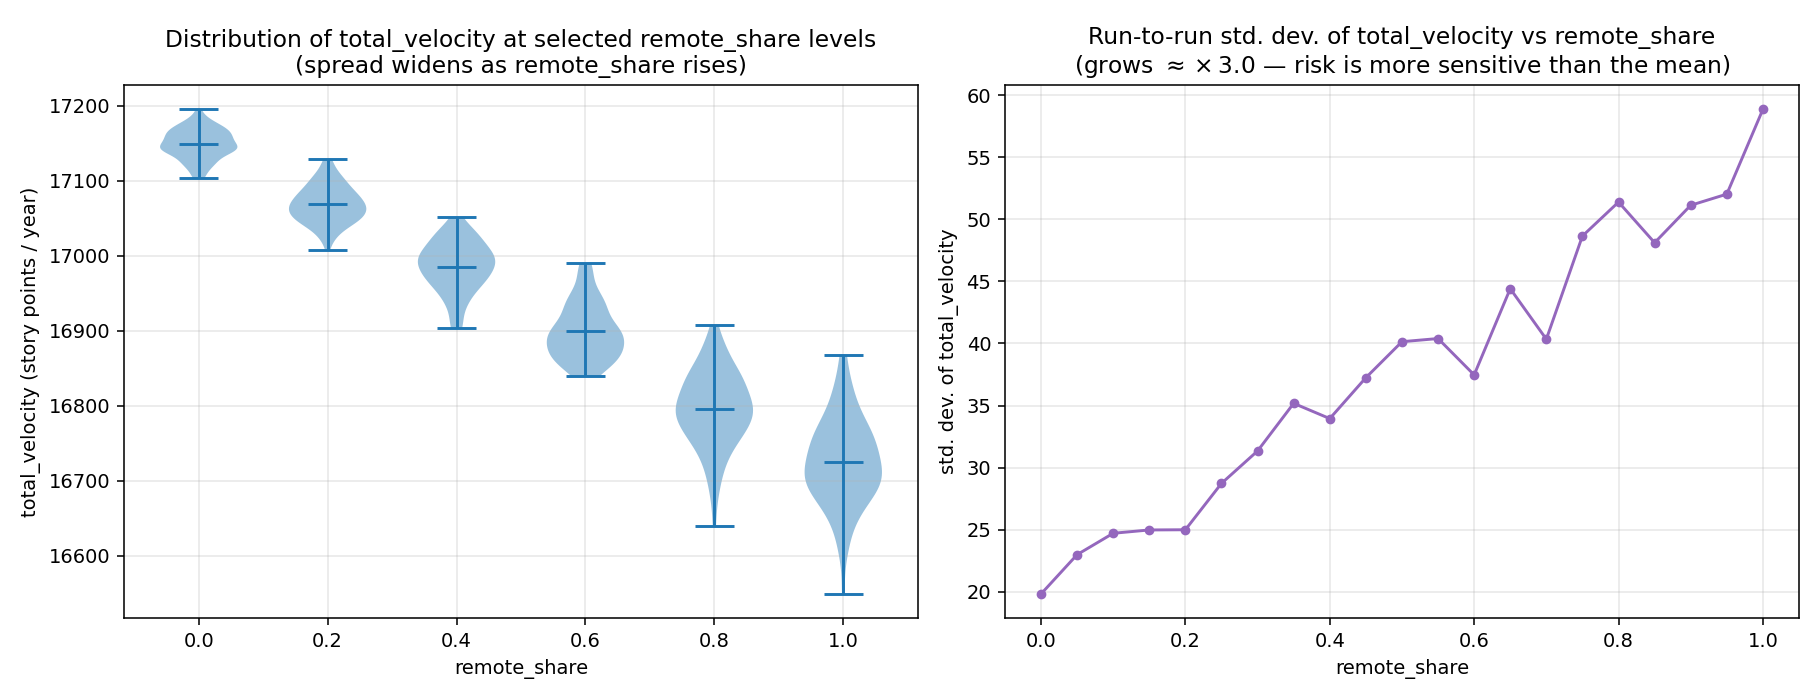
\includegraphics[width=0.62\textwidth]{sens_fig2_dispersion.png}
\caption{Spread of yearly throughput at each level (left) and its run-to-run standard deviation
(right). The mean barely changes, but the spread grows about threefold.}
\label{fig:disp}
\end{figure}

\section{The interactive interface}
\label{sec:ui}

The model is driven through an interactive Streamlit application (\texttt{app\_streamlit.py}, run
with \texttt{streamlit run app\_streamlit.py}). The page uses a wide layout split into a parameter
\emph{sidebar} on the left and a main area on the right that holds an animated view of the team
followed by five metric charts. Changing any parameter re-runs the simulation and redraws everything.
This section documents the whole interface: every parameter, the run-and-replay architecture, the
animation, and each chart.

\subsection{The parameter sidebar}

The sidebar groups every model parameter into collapsible sections by role; the \emph{Headline}
group is expanded by default and the rest start collapsed. Each control is a slider with the default
and range given in Table~\ref{tab:ui-params}. The headline variable is \texttt{remote\_share}; the
remaining groups set up the team's heterogeneity, the work process, learning, turnover, the run's
structure, and reproducibility.

{\footnotesize
\setlength{\tabcolsep}{5pt}
\setlength{\LTleft}{0pt plus 1fill}\setlength{\LTright}{0pt plus 1fill}
\begin{longtable}{llp{8.2cm}}
\caption{The complete sidebar: every parameter exposed by the Streamlit interface, with its default,
range, and what it controls.}\label{tab:ui-params}\\
\toprule
Parameter & Default (range) & What it controls \\
\midrule
\endfirsthead
\multicolumn{3}{l}{\itshape\small Table~\ref{tab:ui-params} (continued)}\\[2pt]
\toprule
Parameter & Default (range) & What it controls \\
\midrule
\endhead
\midrule
\multicolumn{3}{r}{\itshape\small continued on next page}\\
\endfoot
\bottomrule
\endlastfoot
\multicolumn{3}{l}{\textit{Headline}}\\
\texttt{remote\_share} & 0.5 (0--1) & Probability each developer works from home on a given day, rolled afresh every morning. The policy variable under study. \\
\addlinespace
\multicolumn{3}{l}{\textit{Team heterogeneity}}\\
\texttt{mean\_solo\_skill} & 0.5 (0--1) & Team-mean solo skill: the chance a developer clears a blocker alone, without asking for help. \\
\texttt{solo\_skill\_spread} & 0.2 (0--0.5) & Half-width of the uniform spread of solo skill across developers, around the mean. \\
\addlinespace
\multicolumn{3}{l}{\textit{Process}}\\
\texttt{block\_prob} & 0.02 (0--0.10) & Per-tick probability that a working developer hits a blocker. \\
\texttt{sync\_help\_mean} & 1 (0--5) & Mean length, in ticks, of a co-located (office-to-office) help session. \\
\texttt{async\_help\_mean} & 5 (1--20) & Mean length, in ticks, of a help session involving anyone working from home. \\
\addlinespace
\multicolumn{3}{l}{\textit{Learning}}\\
\texttt{learning\_rate} & 0.0123 (0--0.05) & Size of the skill step taken on each learning event; set to 0 to switch learning off. \\
\texttt{skill\_cap} & 0.90 (0.5--1.0) & Ceiling that solo skill approaches but never exceeds. \\
\texttt{sync\_help\_weight} & 1.5 (0--3) & Multiplier on the skill gained when a blocker is resolved through co-located help. \\
\texttt{async\_help\_weight} & 1.0 (0--3) & Same multiplier for remote help; lower than the sync weight, so remote help teaches less. \\
\addlinespace
\multicolumn{3}{l}{\textit{Turnover}}\\
\texttt{annual\_attrition} & 0.12 (0--0.30) & Annual probability that a developer leaves, converted internally to a per-sprint hazard. \\
\texttt{junior\_mean\_skill} & 0.40 (0--0.8) & Skill of a newly hired replacement, as a fraction of the skill ceiling. \\
\texttt{remote\_attrition\_coef} & 0.0 ($-1$--1) & Sign and size of remote work's effect on leaving: positive raises attrition with remote share (isolation), negative lowers it (retention). \\
\addlinespace
\multicolumn{3}{l}{\textit{Structural}}\\
\texttt{n\_devs} & 5 (2--10) & Number of developers on the team. \\
\texttt{sprint\_length} & 320 (32--640) & Ticks per sprint; 320 is ten working days at 32 ticks (15 minutes each) per day. \\
\texttt{n\_sprints} & 24 (1--52) & Number of sprints in the run; 24 two-week sprints is about a year. \\
\texttt{sp\_scaling\_k} & 4 (1--16) & Ticks of work per story point. \\
\addlinespace
\multicolumn{3}{l}{\textit{Reproducibility}}\\
\texttt{seed} & 42 (0--10000) & Random-number seed; fixing it makes a run exactly repeatable. \\
\end{longtable}
}

Below these groups, separated by a divider, sits one control that belongs to the display rather than
to the model: an \emph{animation-frames} slider (100--1000, default 300) that caps how many ticks are
captured for the animation. A long horizon is sub-sampled down to this many frames so that the
playback stays responsive in the browser; finer sub-sampling gives smoother motion at a higher cost.

\subsection{Run-once-then-replay architecture}

Streamlit cannot animate a model while it is stepping, so the run and the playback are deliberately
separated. On any change of parameters the model is executed once to completion and the state of every
developer (activity, location, skill, and any active help session) is snapshotted at each captured
tick. The resulting sequence of frames is then handed to Plotly, whose native play/pause buttons and
time slider replay it entirely in the browser, with no recomputation while scrubbing. The whole run is
cached on the parameter set (\texttt{st.cache\_data}), so moving the slider or pressing play never
re-runs the simulation; only changing a parameter does.

\subsection{The animated team view}

\begin{figure}[ht]
  \centering
  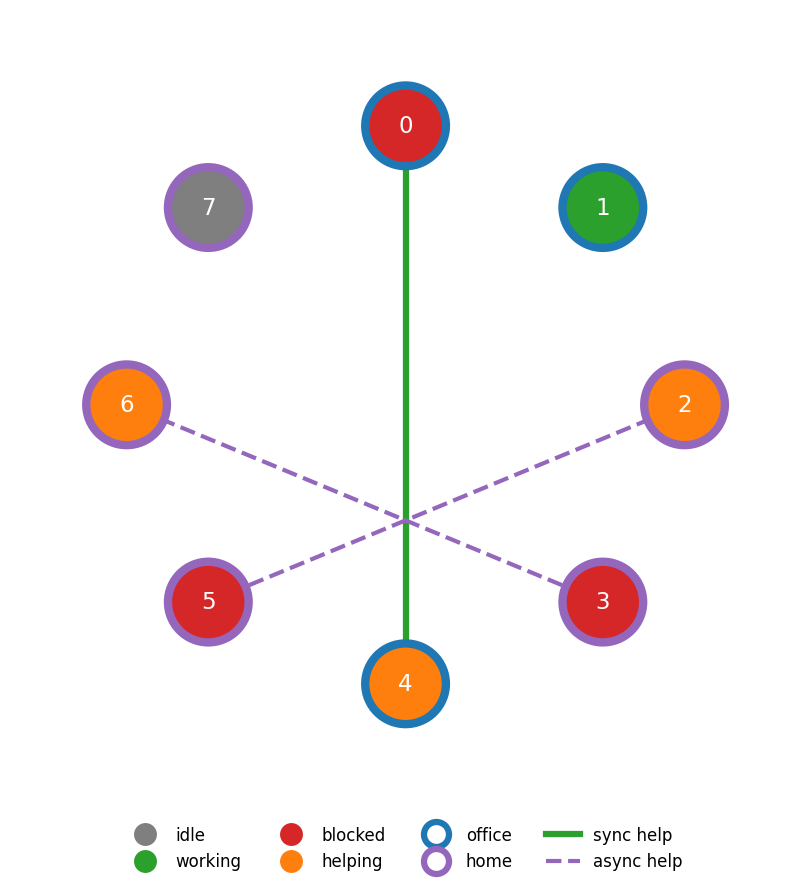
\includegraphics[width=0.48\textwidth]{interface_screenshot.png}
  \caption{A single tick of the animated team view. Inner fill is the developer's state and the outer
  ring is their location; a solid green edge is a co-located (sync) help session and a dashed purple
  edge a remote (async) one. Here a developer is being helped in the office while others, working from
  home, wait on slower asynchronous help.}
  \label{fig:ui}
\end{figure}

Each developer is drawn as a node evenly spaced around a circle, labelled by its slot index
(Figure~\ref{fig:ui}). A node carries two independent colour channels. Its \emph{inner fill} encodes
what the developer is doing this tick: idle (grey), working (green), blocked (red), or helping
someone else (orange). Its \emph{outer ring} encodes where the developer is working today: in the
office (blue) or from home (purple). Location is given its own visual channel because it is the single
distinction that decides whether a help session is fast and co-located or slow and asynchronous.
Hovering a node reveals its index, state, location, and current solo skill.

When one developer is blocked and another steps in to help, an \emph{edge} is drawn between the two
nodes for as long as the session lasts. The edge is a solid green line when both people are in the
office (a synchronous session) and a dashed purple line when at least one is remote (an asynchronous
one). A compact colour legend above the figure maps every fill, ring, and edge style. At a glance the
picture therefore shows how much of the team is productive versus waiting, how the office/home split
falls on any given day, and how much of the help that is happening is the slower remote kind: the
very quantities whose averages drive the velocity and waiting-time curves below.

\subsection{The metric charts}

Below the animation, the main area shows five time-series charts read straight from the model's data
collector and laid out in two columns (Table~\ref{tab:ui-charts}). Together they connect the
micro-level animation to the macro-level outcomes studied in the rest of the report: the velocity and
waiting-time curves are the headline outputs, the developer-states curve is the aggregate of the node
fills, and the skill and attrition curves expose the slower learning and turnover mechanisms.

{\footnotesize
\setlength{\tabcolsep}{5pt}
\setlength{\LTleft}{0pt plus 1fill}\setlength{\LTright}{0pt plus 1fill}
\begin{longtable}{p{4.6cm}p{10.4cm}}
\caption{The five metric charts, all drawn from the data collector over ticks.}\label{tab:ui-charts}\\
\toprule
Chart & What it shows \\
\midrule
\endfirsthead
\multicolumn{2}{l}{\itshape\small Table~\ref{tab:ui-charts} (continued)}\\[2pt]
\toprule
Chart & What it shows \\
\midrule
\endhead
\midrule
\multicolumn{2}{r}{\itshape\small continued on next page}\\
\endfoot
\bottomrule
\endlastfoot
Per-sprint velocity & Story points completed inside the current sprint, resetting to zero at each sprint boundary; the saw-tooth height is that sprint's throughput. \\
Mean waiting time per resolved blocker & Running mean of the ticks between hitting a blocker and clearing it. It rises with the share of remote work, as more help arrives through the slower asynchronous channel. \\
Developer states over time & Number of developers in each state each tick (working, blocked, helping, idle), using the same colours as the node fills in the animation. \\
Team skill over time & Mean, minimum, and maximum solo skill across the team. The upward ramp is learning; the downward steps are turnover, as an experienced leaver is replaced by a low-skill junior. \\
Attrition and tenure & Cumulative number of departures and the team's mean tenure (ticks since each current member was hired). \\
\end{longtable}
}

\section{Implementation and methods}
\label{sec:impl}

\subsection{Software and code organisation}

The model is implemented in Python on top of Mesa~3.x, the standard agent-based-modelling
framework; figures are rendered with Matplotlib, the network animation with Plotly, and the
interactive front-end with Streamlit. The code separates the simulation itself from everything
that drives or observes it (Table~\ref{tab:code}): one self-contained model module, a set of
command-line experiment harnesses, analysis and plotting scripts, and a test suite. The whole
model is about 560 lines; no run depends on any state outside its own \texttt{TeamModel} instance.
The complete source code --- the model, the experiment harnesses, the analysis scripts, and the
test suite --- is available in a public repository at
\url{https://github.com/milolew/sprint-velocity-simulation}.

\begin{table}[H]
\centering
\caption{Code organisation: the simulation is isolated from the harnesses that drive it and the
scripts that analyse its output.}
\label{tab:code}
\small
\setlength{\tabcolsep}{6pt}
\begin{tabular}{p{3.5cm}p{9.4cm}}
\toprule
File & Role \\
\midrule
\texttt{model.py} & Core ABM: \texttt{TeamModel} (Mesa \texttt{Model}), \texttt{Dev} (Mesa \texttt{Agent}), and \texttt{Task} (a passive dataclass). \\
\texttt{experiment.py} & Generic \texttt{remote\_share} sweep harness; each run yields one summary-metrics row. \\
\texttt{run\_experiments.py} & The three single-sprint sweeps of Part~A (baseline, $\times$skill, $\times$blocker rate). \\
\texttt{run\_extended.py}, \texttt{analyze\_extended.py} & The four year-long sweeps of Part~B. \\
\texttt{sensitivity\_remote.py} & Parallel one-parameter sensitivity study; raw per-run output. \\
\texttt{calibrate\_learning.py} & Fits \texttt{learning\_rate} to the literature ramp-up curve. \\
\texttt{plot\_*.py}, \texttt{analyze*.py} & Aggregation (means, CIs) and figure rendering. \\
\texttt{app\_streamlit.py} & Interactive front-end over the same model. \\
\texttt{tests/} & \texttt{pytest} suite (125 tests across 14 files). \\
\bottomrule
\end{tabular}
\end{table}

\subsection{Simulation engine}

A run advances tick by tick. On each tick the model re-rolls daily office/home locations at day
boundaries, closes the sprint and resolves turnover at sprint boundaries, and then activates the
agents. Activation is deliberately \emph{two-phase}: in the first pass every developer that is not
currently seeking help takes its action (work, idle pick-up, solo attempt, help-session tick), and
in the second pass the help-seekers each choose a helper from the now-stable pool of available
colleagues. Without this split, whether a recruited helper had already worked that tick would depend
on the random order in which agents were visited, making runs irreproducible.

Reproducibility is treated as a contract. A run is driven by a single seeded random stream (Mesa's
\texttt{Model(seed=\ldots)}), and every stochastic step consumes a fixed number of draws in a fixed
order regardless of outcome: turnover, for instance, performs exactly one draw per developer in list
order whether or not anyone leaves. A given parameter set and seed therefore reproduce a run exactly,
which the test suite checks directly. Learning, by contrast, is fully deterministic: the bounded
geometric update toward \texttt{skill\_cap} uses no randomness, so its trajectory is identical across
seeds. Each tick a Mesa \texttt{DataCollector} records about sixteen macroscopic reporters (velocity,
mean wait, the per-state head-counts, team skill, attrition, mean tenure, and so on), which are the
series plotted in the interface and aggregated by the analysis scripts. Parameters are validated at
construction, so out-of-range values fail fast rather than propagating into a run.

\subsection{Experimental method and testing}

Every experiment follows the same Monte-Carlo pattern: each parameter cell is run for many
replications under distinct, deterministic seeds (a reproducible function of the cell and replication
index), and the \emph{raw per-run} results are written to CSV so that the full run-to-run
distribution, not just its mean, survives for later analysis. Aggregation and figure rendering live
in separate scripts, so the same CSVs can be re-analysed without re-running the model. The
single-sprint and year-long sweeps run sequentially; the sensitivity study, far larger at roughly
$3{,}000$ runs, is parallelised across worker processes with Python's \texttt{multiprocessing}, each
worker executing one independent simulation. Correctness is guarded by a \texttt{pytest} suite of 125
tests across fourteen files, covering the state machine and blocker handling, the
synchronous/asynchronous help channels, the learning and turnover mechanics, multi-sprint horizons,
the two-phase activation, data collection, parameter validation, and edge cases, with a dedicated
group asserting bit-for-bit determinism under a fixed seed.

\section{Discussion and conclusions}
\label{sec:disc}

The model does not deliver a verdict that remote work is simply good or bad for output. Its central
result is that the cost of remote work is \emph{contingent on the state of the team}. Pulling the
threads together:

\begin{itemize}
\item \textbf{The remote penalty is a tax on the help channel.} Over a single sprint it scales with
how heavily that channel is used: small ($-3.6\%$) for a high-skill team, large ($-13.2\%$) for a
team that blocks frequently. A team that rarely needs help barely notices remote work; a junior,
blocker-heavy team pays dearly.
\item \textbf{Learning attenuates the penalty rather than compounding it.} Over a year the office
advantage is only $\sim$$2.5\%$ and is front-loaded, because as both teams climb the learning curve
they use the penalised help channel less. This emergent reversal of the naive prior is a direct
argument for the agent-based method over a static estimate.
\item \textbf{The decision-relevant effect is on risk, not on the mean.} Going fully remote leaves
expected yearly output almost unchanged but makes it about three times less predictable. A
recommendation based on averages alone would miss the variable that a risk-aware manager cares about.
\item \textbf{Retention is the open question.} Whether remote work helps or harms retention is
genuinely unresolved in the literature; the model carries both readings as named scenarios rather than
choosing one, and over multiple years this channel could dominate the throughput effect studied here.
\end{itemize}

A practical reading is therefore conditional rather than universal: remote work is cheap for a mature,
stable, high-skill team and costly for a junior-heavy, high-churn team that is still onboarding, where
the cost front-loads exactly when the team can least afford it.

\paragraph{Limitations and next steps.} No published source measures the model's exact constructs, so
the parameters are reconstructions and the results should be read as the shape of a response, not as
calibrated forecasts. The model uses a single, undifferentiated \texttt{remote\_attrition\_coef} and
so cannot capture the seniority-conditioning the literature shows; the learning-channel coupling is
muted at the default low blocker rate and would become material only in a blocker-heavy or
junior-heavy regime. The clearest next step is a full sweep of \texttt{remote\_attrition\_coef} over
$[-1,1]$, which would couple retention back into the skill channel over a multi-year horizon and
plausibly dominate the $2.5\%$ throughput effect measured here.

\begin{thebibliography}{9}
\small

\bibitem{proximity} N.~Emanuel, E.~Harrington, and A.~Pallais.
\emph{The Power of Proximity to Coworkers: Training for Tomorrow or Productivity Today?}
NBER Working Paper 31880, 2023.

\bibitem{remotely} N.~Emanuel and E.~Harrington.
\emph{Working Remotely? Selection, Treatment, and the Market for Remote Work.}
American Economic Journal: Applied Economics, 16(4), 2024.

\bibitem{bloom} N.~Bloom, R.~Han, and J.~Liang.
\emph{Hybrid working from home improves retention without damaging performance.}
Nature, 630, 2024.

\bibitem{gibbs} M.~Gibbs, F.~Mengel, and C.~Siemroth.
\emph{Work from Home and Productivity: Evidence from Personnel and Analytics Data on IT Professionals.}
Journal of Political Economy Microeconomics, 2023.

\bibitem{yang} L.~Yang, D.~Holtz, S.~Jaffe, et al.
\emph{The effects of remote work on collaboration among information workers.}
Nature Human Behaviour, 5, 2021.

\bibitem{dieste} O.~Dieste, A.~M.~Aranda, F.~Uyaguari, et al.
\emph{Empirical evaluation of the effects of experience on code quality and programmer productivity.}
Empirical Software Engineering, 22(5), 2017.

\bibitem{peitek} N.~Peitek, S.~Apel, C.~Parnin, A.~Brechmann, and J.~Siegmund.
\emph{Program Comprehension and Code Complexity Metrics: An fMRI Study.}
ESEC/FSE, 2022.

\bibitem{mcconnell} A.~Oram and G.~Wilson (eds.).
\emph{Making Software: What Really Works, and Why We Believe It} (ch.~30, on Sackman et al.~1968).
O'Reilly, 2010.

\bibitem{bls} U.S.~Bureau of Labor Statistics.
\emph{Job Openings and Labor Turnover Survey (JOLTS)} and \emph{Employee Tenure}, 2024.

\bibitem{mesa} J.~Kazil, D.~Masad, and A.~Crooks.
\emph{Utilizing Python for Agent-Based Modeling: The Mesa Framework.}
SBP-BRiMS, 2020.

\end{thebibliography}

\end{document}
